%!TEX program = xelatex
\documentclass[aspectratio=169,10pt]{ctexbeamer}
\usepackage[bluetheme]{ustcbeamer}
% !TeX root = ./main.tex

% 自适应16:9的宽高比设置
\makeatletter
\@ifclasswith{ctexbeamer}{aspectratio=169}{
		\def\backxscale{4/3}\def\backyscale{1}\def\ustcshift{30}
	}{
		\def\backxscale{1.068}\def\backyscale{1.068}\def\ustcshift{0}
	}
\makeatother

\newcommand{\maketitleframe}{
	%取消footline,sidebar
	\setbeamertemplate{footline}[footlineoff]
	%%设置本命令以后的背景如下
	\usebackgroundtemplate{%
			% !TeX root = ./main.tex
\begin{tikzpicture}[y=1pt, x=1pt, yscale=0.474*\backyscale, xscale=0.474*\backxscale, inner sep=0pt, outer sep=0pt]
    % \begin{scope}[cm={{1,0.0,0.0,-1,(0,0)}}]
      \path[fill=themecolor1,even odd rule] (720.4059,0.3515) -- (720.4059,71.1507) --
        (0.3436,71.1507) -- (0.3436,0.3515) -- cycle;
    
    
    
      \path[fill=themecolor2,even odd rule] (0.3436,76.0927) -- (720.4059,76.0927) --
        (720.4059,79.3043) -- (0.3436,79.3043) -- cycle;
    
    
    
      \path[left color=themecolor!80, right color=themecolor,even odd rule] (720.4059,392.4714) -- (0.3436,392.4714) --
        (0.3436,112.2780) -- (720.4059,112.2780) -- cycle;
    
    
    
          \path[even odd rule] (720.4059,392.4714) -- (0.3436,392.4714) --
            (0.3436,112.2780) -- (720.4059,112.2780) -- cycle;
    
    
    
      \path[fill=themecolor1,even odd rule] (0.3436,540.3980) -- (720.4059,540.3980) --
        (720.4059,433.5987) -- (0.3436,433.5987) -- cycle;
    
    
    
      \path[fill=themecolor,even odd rule] (84.0129,392.4714) -- (64.1007,392.4714) ..
        controls (139.6636,296.8146) and (237.7485,213.1007) .. (369.3679,152.9909) ..
        controls (258.0055,213.1787) and (160.4523,292.5573) .. (84.0129,392.4714) --
        cycle(0.3436,210.9419) -- (0.3436,112.2780) -- (205.1827,112.2780) .. controls
        (135.2103,142.0132) and (67.0535,175.1304) .. (0.3436,210.9419) --
        cycle(0.3436,318.0849) -- (0.3436,261.2429) .. controls (87.4868,197.7318) and
        (173.6552,147.4217) .. (257.6874,112.2780) -- (329.6364,112.2780) .. controls
        (208.4627,165.2559) and (97.0387,225.2988) .. (0.3436,318.0849) --
        cycle(23.7974,392.4714) -- (0.3436,392.4714) -- (0.3436,375.5798) .. controls
        (103.8628,248.3597) and (243.0859,163.2623) .. (385.7678,112.2780) --
        (411.7601,112.2780) .. controls (266.1313,174.0682) and (125.2848,246.4444) ..
        (23.7974,392.4714);
    
    
    
      \path[fill=themecolor2,even odd rule] (0.3436,428.6568) -- (720.4059,428.6568) --
        (720.4059,425.4452) -- (0.3436,425.4452) -- cycle;

      \node at(185-\ustcshift,488){\textcolor{themecolor}{
\includegraphics[scale=1]{./theme/ustc_logo_side.pdf}}};
    % \end{scope}
\end{tikzpicture}
	}%
	%封面页
	\begin{frame}%
		\maketitle%
	\end{frame}%
	%设置本命令以后的背景如下
	\usebackgroundtemplate{%
			% !TeX root = ./main.tex
\begin{tikzpicture}[y=1pt, x=1pt, yscale=0.474*\backyscale, xscale=0.474*\backxscale, inner sep=0pt, outer sep=0pt]
% \begin{scope}[cm={{1,0.0,0.0,-1,(0,0)}}]
    \path[left color=themecolor!80,right color=themecolor,even odd rule] (720.4059,540.3980) -- (0.3436,540.3980) --
      (0.3436,478.8258) -- (720.4059,478.8258) -- cycle;



        \path[even odd rule] (720.4059,540.3980) -- (0.3436,540.3980) --
          (0.3436,478.8258) -- (720.4059,478.8258) -- cycle;



    \path[fill=themecolor,even odd rule] (84.0129,540.3980) -- (64.1007,540.3980) ..
      controls (139.6636,519.3777) and (237.7485,500.9814) .. (369.3679,487.7725) ..
      controls (258.0055,500.9987) and (160.4523,518.4420) .. (84.0129,540.3980) --
      cycle(0.3436,500.5071) -- (0.3436,478.8258) -- (205.1827,478.8258) .. controls
      (135.2103,485.3599) and (67.0535,492.6376) .. (0.3436,500.5071) --
      cycle(0.3436,524.0517) -- (0.3436,511.5606) .. controls (87.4868,497.6042) and
      (173.6552,486.5485) .. (257.6874,478.8258) -- (329.6364,478.8258) .. controls
      (208.4627,490.4677) and (97.0387,503.6621) .. (0.3436,524.0517) --
      cycle(23.7974,540.3980) -- (0.3436,540.3980) -- (0.3436,536.6860) .. controls
      (103.8628,508.7296) and (243.0859,490.0294) .. (385.7678,478.8258) --
      (411.7601,478.8258) .. controls (266.1313,492.4040) and (125.2848,508.3087) ..
      (23.7974,540.3980);

  \path[fill=themecolor2,even odd rule] (720.4059,475.6141) -- (0.3436,475.6141) --
    (0.3436,478.8258) -- (720.4059,478.8258) -- cycle;



  \path[fill=themecolor,even odd rule] (0.3436,0.3515) -- (720.4059,0.3515) --
    (720.4059,28.5100) -- (0.3436,28.5100) -- cycle;



  \path[fill=themecolor2,even odd rule] (720.4059,28.5100) -- (0.3436,28.5100) --
    (0.3436,31.7217) -- (720.4059,31.7217) -- cycle;

  \node at(580+\ustcshift,509){\textcolor{white}{
\includegraphics[scale=0.8]{./theme/ustc_logo_side.pdf}}};



% \end{scope}

\end{tikzpicture}
	}%
}%
%
\usepackage{booktabs,graphicx,amsmath,array,tabularx}
\usepackage{hyperref}
\usepackage{tikz}
\usetikzlibrary{arrows.meta,positioning,fit,calc}
\setbeamertemplate{navigation symbols}{}
\newcommand{\paperref}[1]{\par\vfill{\raggedleft\scriptsize #1\par}}
\title[AEL-YOLO]{You Only Look Once Meets Asymmetric Pronged Convolution}
\subtitle{面向 RGB 火焰与烟雾检测的统一框架}
\author[组会汇报]{组会论文汇报}
\institute{Engineering Applications of Artificial Intelligence, 173 (2026), 114484}
\date{2026 年 10 月 23 日}
\begin{document}
\maketitleframe
\setbeamertemplate{footline}{%
  \leavevmode\hfill\insertshorttitle\hspace{1em}\insertframenumber/\inserttotalframenumber\hspace{0.7cm}\vspace{0.15cm}%
}
\setbeamercolor{footline}{fg=white,bg=themecolor}

\begin{frame}{论文与期刊：EAAI 的中科院分区}
\begin{columns}[T,onlytextwidth]
\begin{column}{.62\textwidth}
{\Large\bfseries Engineering Applications of Artificial Intelligence}
\vspace{.12cm}

\small Elsevier 旗下同行评审期刊，关注人工智能在工程领域的实际应用。
\vspace{.4cm}

\begin{block}{中科院分区（2025 年升级版）}
大类“计算机科学”1 区，TOP 期刊；小类“工程：综合”1 区。“自动化与控制系统”“计算机：人工智能”“工程：电子与电气”均为 2 区。
\end{block}
\begin{block}{这篇文章的开放获取状态}
该刊为订阅期刊；本文在 ScienceDirect 页面显示“Get rights and content”，按非 OA 论文介绍。
\end{block}
\end{column}
\begin{column}{.34\textwidth}
\centering
\begin{tikzpicture}[node distance=7mm,every node/.style={draw=themecolor,rounded corners,align=center,minimum width=3.2cm,minimum height=.85cm,font=\small}]
\node[fill=themecolor!10] (journal) {EAAI\\工程应用 + 人工智能};
\node[fill=blue!7,below=of journal] (index) {中科院大类\\计算机科学 1 区 / TOP};
\node[fill=orange!12,below=of index] (paper) {本文：非 OA\\2026 年，第 173 卷};
\draw[-{Latex},thick,themecolor] (journal)--(index);
\draw[-{Latex},thick,themecolor] (index)--(paper);
\end{tikzpicture}
\end{column}
\end{columns}
\vfill\tiny 分区依据：中科院期刊分区表 2025 年升级版；论文出版信息与访问状态：Elsevier ScienceDirect，doi:10.1016/j.engappai.2026.114484。
\end{frame}

\begin{frame}{从火灾预警到图像检测：烟雾是早期线索}
\begin{columns}[T,onlytextwidth]
\begin{column}{.53\textwidth}
\begin{itemize}
\item 温度、烟感等传感器容易受环境影响，初期响应也可能滞后。
\item RGB 摄像头可覆盖较大区域，直接给出火焰和烟雾的位置。
\item 烟雾常低对比、半透明、边界扩散；云、尘、蒸汽也可能与烟相似。
\item 远处烟团像素少，遮挡和光照变化进一步增加漏检、误报风险。
\end{itemize}
\end{column}
\begin{column}{.43\textwidth}
\centering
\begin{tikzpicture}[scale=.78,transform shape,node distance=5mm, every node/.style={align=center,font=\small}]
\node[draw=themecolor,rounded corners,fill=themecolor!8,minimum width=3.6cm,minimum height=0.8cm] (cam) {RGB 图像};
\node[draw=themecolor,rounded corners,fill=themecolor!8,below=of cam,minimum width=3.6cm,minimum height=0.8cm] (det) {目标检测模型};
\draw[-{Latex},thick,themecolor] (cam) -- (det);
\node[draw=blue!55,rounded corners,fill=blue!7,below left=5mm and -3mm of det,minimum width=2.15cm,minimum height=0.85cm] (fire) {Fire box};
\node[draw=orange!75!black,rounded corners,fill=orange!12,below right=5mm and -3mm of det,minimum width=2.15cm,minimum height=0.85cm] (smoke) {Smoke box};
\draw[-{Latex},thick,themecolor] (det) -- (fire);
\draw[-{Latex},thick,themecolor] (det) -- (smoke);
\end{tikzpicture}
\end{column}
\end{columns}
\vspace{.25cm}\small 论文聚焦：在实时检测框架中同时识别 Fire 与 Smoke，并降低复杂背景下的混淆。
\end{frame}

\begin{frame}{面对这些背景，论文怎样应对？}
\centering
\renewcommand{\arraystretch}{1.4}
\begin{tabularx}{\textwidth}{>{\raggedright\arraybackslash}p{.29\textwidth} >{\raggedright\arraybackslash}X >{\raggedright\arraybackslash}p{.26\textwidth}}
\toprule
\textbf{背景中的困难} & \textbf{论文的应对方式} & \textbf{对应设计}\\
\midrule
烟雾边缘扩散、形状不规则 & 用不同方向和感受范围的卷积分支提取烟羽纹理 & APConv\\
火焰、烟雾大小差异大，背景也复杂 & 在不同层级融合特征，并让多尺度检测头分别预测 & C2f-AFF、LSADetect\\
真实场景图像来源杂，重复、水印会干扰训练 & 汇集多来源图像并清理数据，发布 Finaldata 与标注 & 数据集整理\\
\bottomrule
\end{tabularx}
\vspace{.5cm}
\begin{block}{用一句话概括}
论文把“看清不同形态的火烟、融合不同尺度的信息、整理训练图像”分别落实到网络模块和数据集构建中。
\end{block}
\small 这是论文设计与背景问题的对应关系；论文没有逐类报告云雾、逆光等条件下的误报率。
\end{frame}

\section{数据与问题}
\begin{frame}{数据质量也是火烟检测问题的一部分}
\begin{columns}[T,onlytextwidth]
\begin{column}{.48\textwidth}
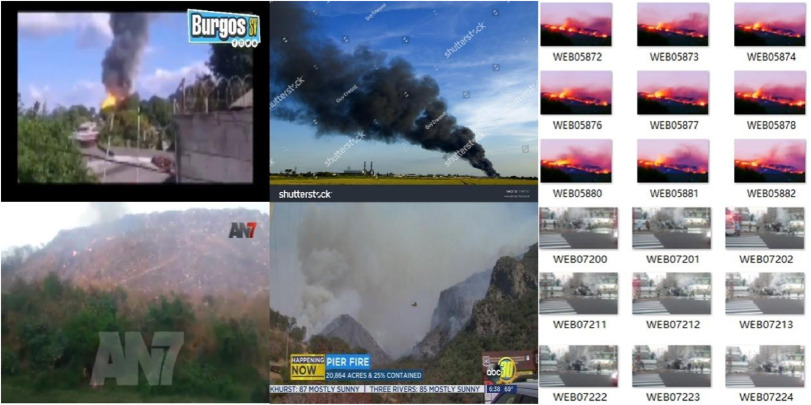
\includegraphics[width=\linewidth]{images/paper_fig6.jpg}
\end{column}
\begin{column}{.47\textwidth}
\begin{itemize}
\item 论文指出，公开图像常有重复样本、水印和来源单一的问题。
\item Finaldata 汇集 D-Fire 与网络图像，覆盖城市、森林等自然场景。
\item 作者称清理了错误、重复和含水印样本，并提供 Fire / Smoke 标注。
\item 多源数据能增加场景变化，但不能自动保证跨地点、跨摄像头泛化。
\end{itemize}
\vspace{.2cm}\small 图中可见网络图像的水印和近重复样本，说明数据整理会影响训练与评估。
\end{column}
\end{columns}
\end{frame}

\begin{frame}{Finaldata：作者划分与本地标签核验}
\centering
\vspace{3pt}
\renewcommand{\arraystretch}{1.25}
\begin{tabular}{lrrr}
\toprule
划分 & 图像数 & Fire 框 & Smoke 框\\ \midrule
Train & 14,244 & 25,868 & 12,985\\
Valid & 2,641 & 3,055 & 1,409\\ \midrule
合计 & 16,885 & 28,923 & 14,394\\
\bottomrule
\end{tabular}
\vspace{.2cm}
\begin{columns}[T,onlytextwidth]
\begin{column}{.48\textwidth}
\begin{itemize}
\item 仓库数据包采用 YOLO 检测标注，类别 ID 为 0=fire、1=smoke。
\item 空标签负样本：Train 1,747 张，Valid 1,001 张。
\end{itemize}
\end{column}
\begin{column}{.48\textwidth}
\begin{itemize}
\item 本地逐项核对图像与标签配对及类别框数量。
\item 发现 13 个宽或高为 0 的退化框，保留原始文件并记录。
\end{itemize}
\end{column}
\end{columns}
\small 本地统计来自作者发布的 train/valid 压缩包；它不是独立采集的外部测试集。
\end{frame}

\begin{frame}{模型总览：骨干提特征，检测头融合多尺度信息}
\centering
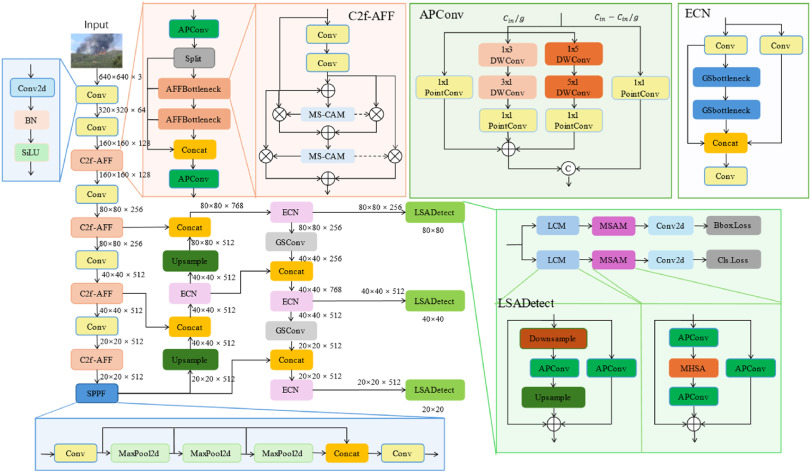
\includegraphics[width=.96\linewidth,height=.77\textheight,keepaspectratio]{images/paper_fig1.jpg}
\par\small 原论文 Figure 1：骨干网络、特征融合路径，以及 APConv、C2f-AFF、ECN、LSADetect 模块。
\end{frame}

\section{方法}
\begin{frame}{APConv：把方形卷积分成横向、纵向分支}
\begin{columns}[T,onlytextwidth]
\begin{column}{.53\textwidth}
\begin{itemize}
\item 普通卷积用固定方形窗口提取局部特征。
\item APConv 并行计算三路：\(1\times5+5\times1\)、\(1\times3+3\times1\)、\(1\times1\)。
\item 前两路先横向再纵向处理，最后与点卷积分支相加。
\item 这样同时保留方向性纹理和不同范围的空间线索，适合形状弥散、细长的火烟区域。
\end{itemize}
\end{column}
\begin{column}{.42\textwidth}
\centering
\begin{tikzpicture}[scale=.78,transform shape,node distance=4mm,every node/.style={font=\small,align=center}]
\node[draw,rounded corners,fill=gray!10,minimum width=2.9cm] (in) {输入特征};
\node[draw,rounded corners,fill=blue!9,below left=6mm and 2mm of in,minimum width=1.55cm] (a) {1×5\;→\;5×1};
\node[draw,rounded corners,fill=blue!9,below=6mm of in,minimum width=1.55cm] (b) {1×3\;→\;3×1};
\node[draw,rounded corners,fill=orange!15,below right=6mm and 2mm of in,minimum width=1.55cm] (c) {1×1};
\node[draw,circle,fill=green!15,below=14mm of b] (sum) {+};
\node[draw,rounded corners,fill=gray!10,below=5mm of sum,minimum width=2.9cm] (out) {融合输出};
\draw[-{Latex}] (in) -- (a); \draw[-{Latex}] (in) -- (b); \draw[-{Latex}] (in) -- (c);
\draw[-{Latex}] (a) -- (sum); \draw[-{Latex}] (b) -- (sum); \draw[-{Latex}] (c) -- (sum); \draw[-{Latex}] (sum) -- (out);
\end{tikzpicture}
\vspace{.2cm}\small 作者代码实现：分组卷积 + BN + SiLU。
\end{column}
\end{columns}
\end{frame}

\begin{frame}{C2f-AFF：保留 C2f 分支，再按特征内容融合}
\begin{columns}[T,onlytextwidth]
\begin{column}{.49\textwidth}
\begin{itemize}
\item C2f 将输入分成多条路径，部分路径经过 Bottleneck，之后拼接。
\item 论文在模块中加入 APConv，并用 AFF/iAFF 在局部与全局分支计算融合权重。
\item 直观理解：浅层细节和更大范围的上下文可以按内容加权后再合并。
\end{itemize}
\end{column}
\begin{column}{.47\textwidth}
\centering
\begin{tikzpicture}[scale=.78,transform shape,node distance=4mm,every node/.style={draw,rounded corners,align=center,font=\small}]
\node[fill=gray!10,minimum width=2.9cm] (x) {输入特征};
\node[fill=blue!9,below left=7mm and 0mm of x,minimum width=1.6cm] (p) {APConv 投影};
\node[fill=blue!9,below right=7mm and 0mm of x,minimum width=1.6cm] (q) {Bottleneck};
\node[fill=orange!14,below=9mm of p,minimum width=1.6cm] (loc) {局部注意力};
\node[fill=orange!14,below=9mm of q,minimum width=1.6cm] (glob) {全局注意力};
\node[fill=green!13,below=8mm of $(loc)!0.5!(glob)$,minimum width=2.9cm] (f) {加权融合 / 拼接};
\draw[-{Latex}] (x)--(p); \draw[-{Latex}] (x)--(q); \draw[-{Latex}] (p)--(loc); \draw[-{Latex}] (q)--(glob); \draw[-{Latex}] (loc)--(f); \draw[-{Latex}] (glob)--(f);
\end{tikzpicture}
\end{column}
\end{columns}
\end{frame}

\begin{frame}{ECN：在特征融合路径上控制计算量}
\begin{columns}[T,onlytextwidth]
\begin{column}{.5\textwidth}
\begin{itemize}
\item Head 需要把高分辨率细节与低分辨率语义反复融合。
\item 论文的 ECN 使用轻量卷积和跨阶段分支处理特征。
\item 作者代码对应模块包含 GSConv 与 VoVGSCSP：部分通道做常规卷积，另一路用较轻操作生成特征，再拼接融合。
\item 设计目标是保留检测需要的信息，同时降低融合层开销。
\end{itemize}
\end{column}
\begin{column}{.45\textwidth}
\centering
\begin{tikzpicture}[scale=.78,transform shape,node distance=5mm,every node/.style={draw,rounded corners,align=center,font=\small}]
\node[fill=gray!10,minimum width=2.8cm] (in) {输入特征};
\node[fill=blue!9,below left=7mm and 0mm of in,minimum width=1.5cm] (dense) {常规卷积};
\node[fill=orange!14,below right=7mm and 0mm of in,minimum width=1.5cm] (cheap) {轻量卷积 + shortcut};
\node[fill=green!13,below=10mm of $(dense)!0.5!(cheap)$,minimum width=2.8cm] (cat) {拼接 / 融合};
\draw[-{Latex}] (in)--(dense); \draw[-{Latex}] (in)--(cheap); \draw[-{Latex}] (dense)--(cat); \draw[-{Latex}] (cheap)--(cat);
\end{tikzpicture}
\vspace{.2cm}\small 模块目标是降计算；实际速度仍由实现、设备和其他层共同决定。
\end{column}
\end{columns}
\end{frame}

\begin{frame}{LSADetect：P3、P4、P5 分别预测框和类别}
\begin{columns}[T,onlytextwidth]
\begin{column}{.53\textwidth}
\begin{itemize}
\item 三种尺度保留不同网格密度：P3 对细小目标更敏感，P5 覆盖更大区域。
\item 每个尺度分开做框回归和类别预测。
\item 作者代码的 Detect\_SA 在两条预测分支中加入 APConv 与 Self-Attention。
\item 注意力让位置之间交换信息；论文提出轻量化设计以兼顾检测效果和推理效率。
\end{itemize}
\end{column}
\begin{column}{.42\textwidth}
\centering
\begin{tikzpicture}[scale=.78,transform shape,node distance=4mm,every node/.style={draw,rounded corners,align=center,font=\small}]
\node[fill=blue!8,minimum width=2.35cm] (p3) {P3：高分辨率};
\node[fill=blue!8,below=of p3,minimum width=2.35cm] (p4) {P4：中分辨率};
\node[fill=blue!8,below=of p4,minimum width=2.35cm] (p5) {P5：低分辨率};
\node[fill=green!12,right=4mm of p4,minimum width=1.25cm] (box) {APConv + Attention};
\node[fill=orange!15,right=4mm of box,minimum width=1.05cm] (out) {框 / 类别};
\draw[-{Latex}] (p3.east) -- (box.west); \draw[-{Latex}] (p4.east) -- (box.west); \draw[-{Latex}] (p5.east) -- (box.west); \draw[-{Latex}] (box) -- (out);
\end{tikzpicture}
\end{column}
\end{columns}
\end{frame}

\section{实验结果}
\begin{frame}{论文结果：准确率提升，同时报告实时速度}
\begin{columns}[T,onlytextwidth]
\begin{column}{.57\textwidth}
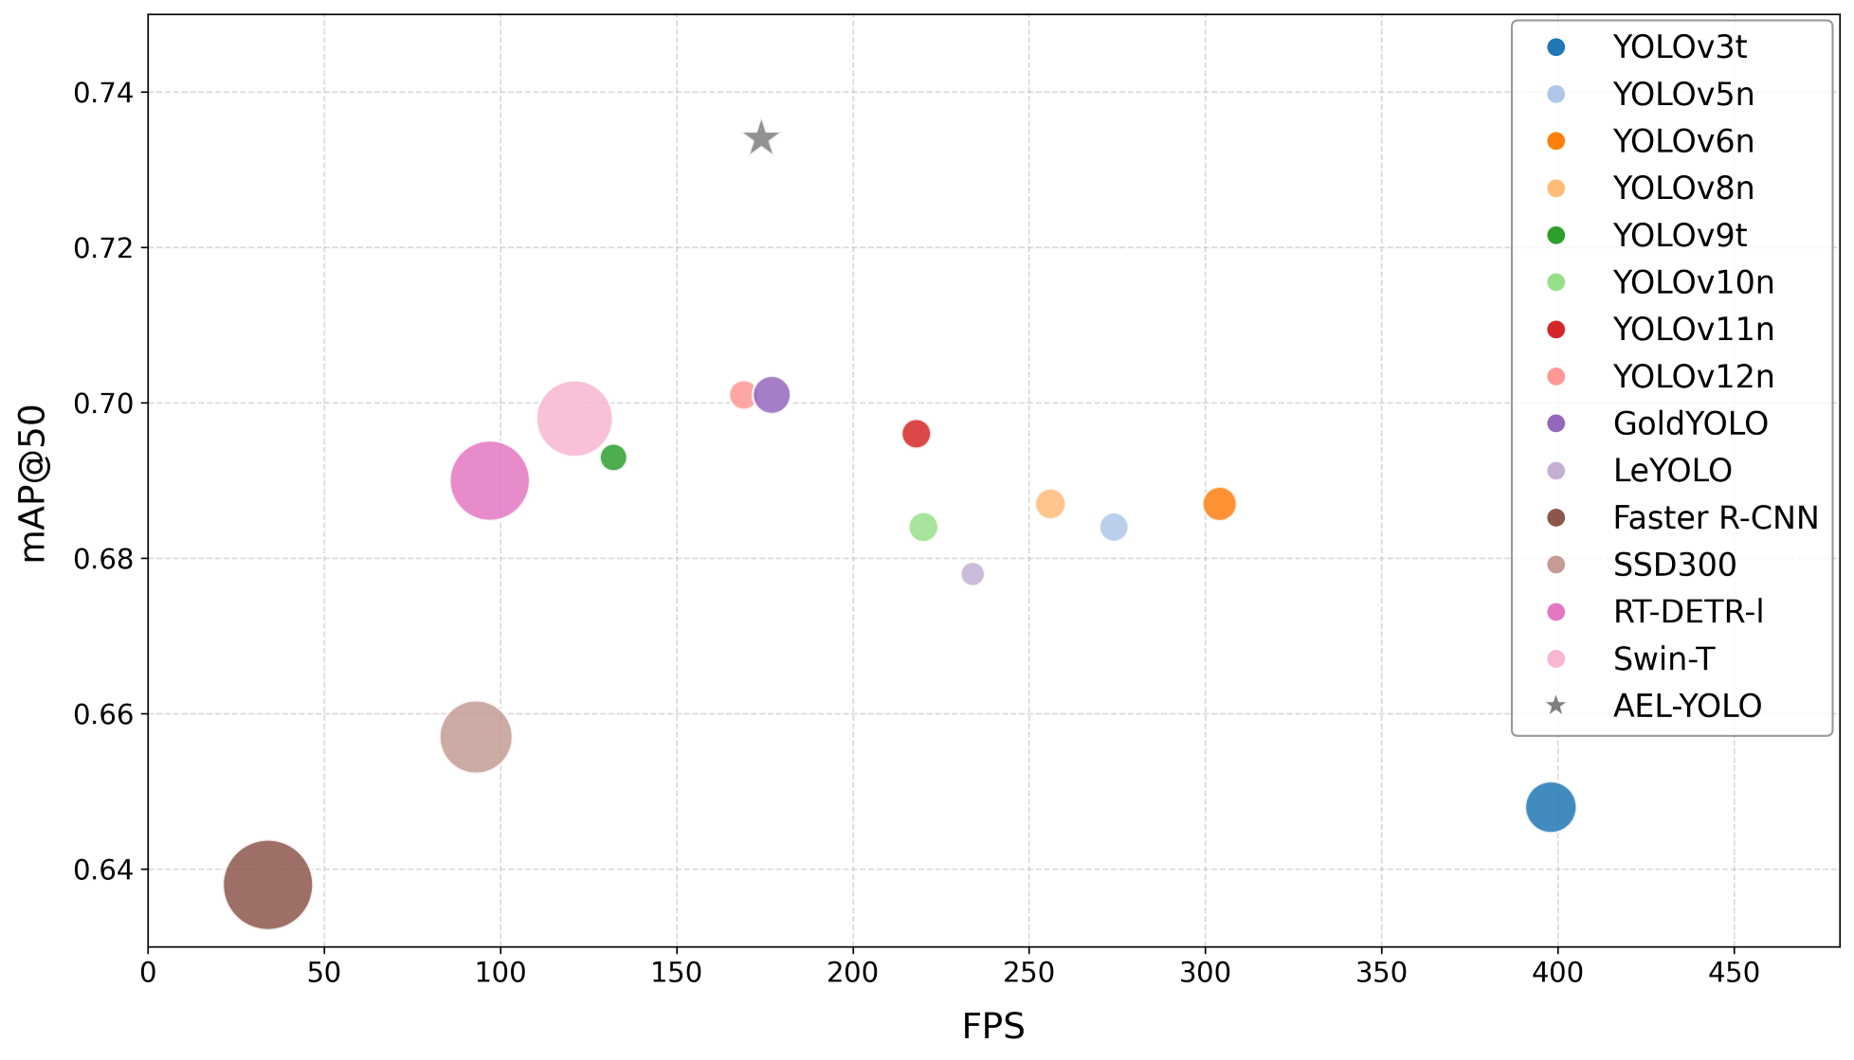
\includegraphics[width=\linewidth]{images/paper_results.png}
\end{column}
\begin{column}{.39\textwidth}
\begin{itemize}
\item Finaldata 上，摘要报告 mAP@0.5 提升 4.7%，mAP@0.5:0.95 提升 4.5%。
\item 摘要报告推理速度 174 FPS。
\item 论文还在两个公开数据集上做补充实验。
\end{itemize}
\vspace{.15cm}\small FPS 受 GPU、输入尺寸、batch 和测速流程影响，不能直接等同于部署延迟。
\end{column}
\end{columns}
\vspace{.1cm}{\scriptsize 图为论文模型比较结果；数字是论文报告，不是本地复现指标。}
\end{frame}

\section{代码复现}
\begin{frame}{YAML 到代码：配置名和 Python 模块如何对应}
\begin{columns}[T,onlytextwidth]
\begin{column}{.49\textwidth}
\textbf{YAML 逐层字段}
\begin{itemize}
\item `from`：取哪一层输出。
\item `repeats`：模块重复次数。
\item `module`：模块类名。
\item `args`：通道数、卷积核、类别数等参数。
\end{itemize}
\texttt{from / repeats / module / args}
\end{column}
\begin{column}{.47\textwidth}
\textbf{当前作者 YAML 中可见的模块}
\begin{itemize}
\item Backbone：Conv、C2f\_iAFF、SPPF。
\item Head：VoVGSCSP、GSConv、Detect\_SA。
\item 自定义实现分布在 `iAFF6.py`、`ECN.py`、`SAhead6.py`。
\item YAML 写网络结构；它不包含训练好的参数权重。
\end{itemize}
\end{column}
\end{columns}
\end{frame}

\begin{frame}{复现配置：沿用作者结构，从随机初始化训练}
\centering
\vspace{3pt}
\renewcommand{\arraystretch}{1.18}
\begin{tabular}{ll}
\toprule
项目 & 本次服务器运行设置\\ \midrule
模型配置 & `C2f-AFF+ECN+LSADetect.yaml`\\
初始化 & `pretrained=False`，不加载预训练权重\\
数据与输入 & Finaldata 作者划分，640 × 640\\
训练计划 & 最多 200 epochs，patience=50，SGD\\
Batch / seed & 40 / 0；deterministic=True\\
设备绑定 & 物理 GPU 3，通过 UUID 绑定\\
\bottomrule
\end{tabular}
\vspace{.22cm}
\begin{itemize}
\item 作者 train.py 使用 batch 16、pretrained=True；本次按需求改为 batch 40、从头训练。
\item 每轮验证开销不会随 batch 同比例下降，因此增大 batch 后总用时不会按比例缩短。
\end{itemize}
\end{frame}

\begin{frame}{复现结果：200 轮完成，验证集 mAP@0.5 为 71.9\%}
\begin{columns}[T,onlytextwidth]
\begin{column}{.47\textwidth}
\begin{block}{best.pt：作者验证划分}
\begin{itemize}
\item 2,641 张图像、4,464 个标注框，其中 1,001 张为无目标背景图。
\item Precision 74.5\%；Recall 64.5\%。
\item mAP@0.5 71.9\%；mAP@0.5:0.95 42.8\%。
\end{itemize}
\end{block}
\vspace{.1cm}
\renewcommand{\arraystretch}{1.12}
\begin{tabular}{lrr}
\toprule
类别 & AP@0.5 & AP@0.5:0.95 \\\midrule
Fire & 68.8\% & 37.9\% \\
Smoke & 75.0\% & 47.7\% \\
\bottomrule
\end{tabular}
\end{column}
\begin{column}{.51\textwidth}
\centering
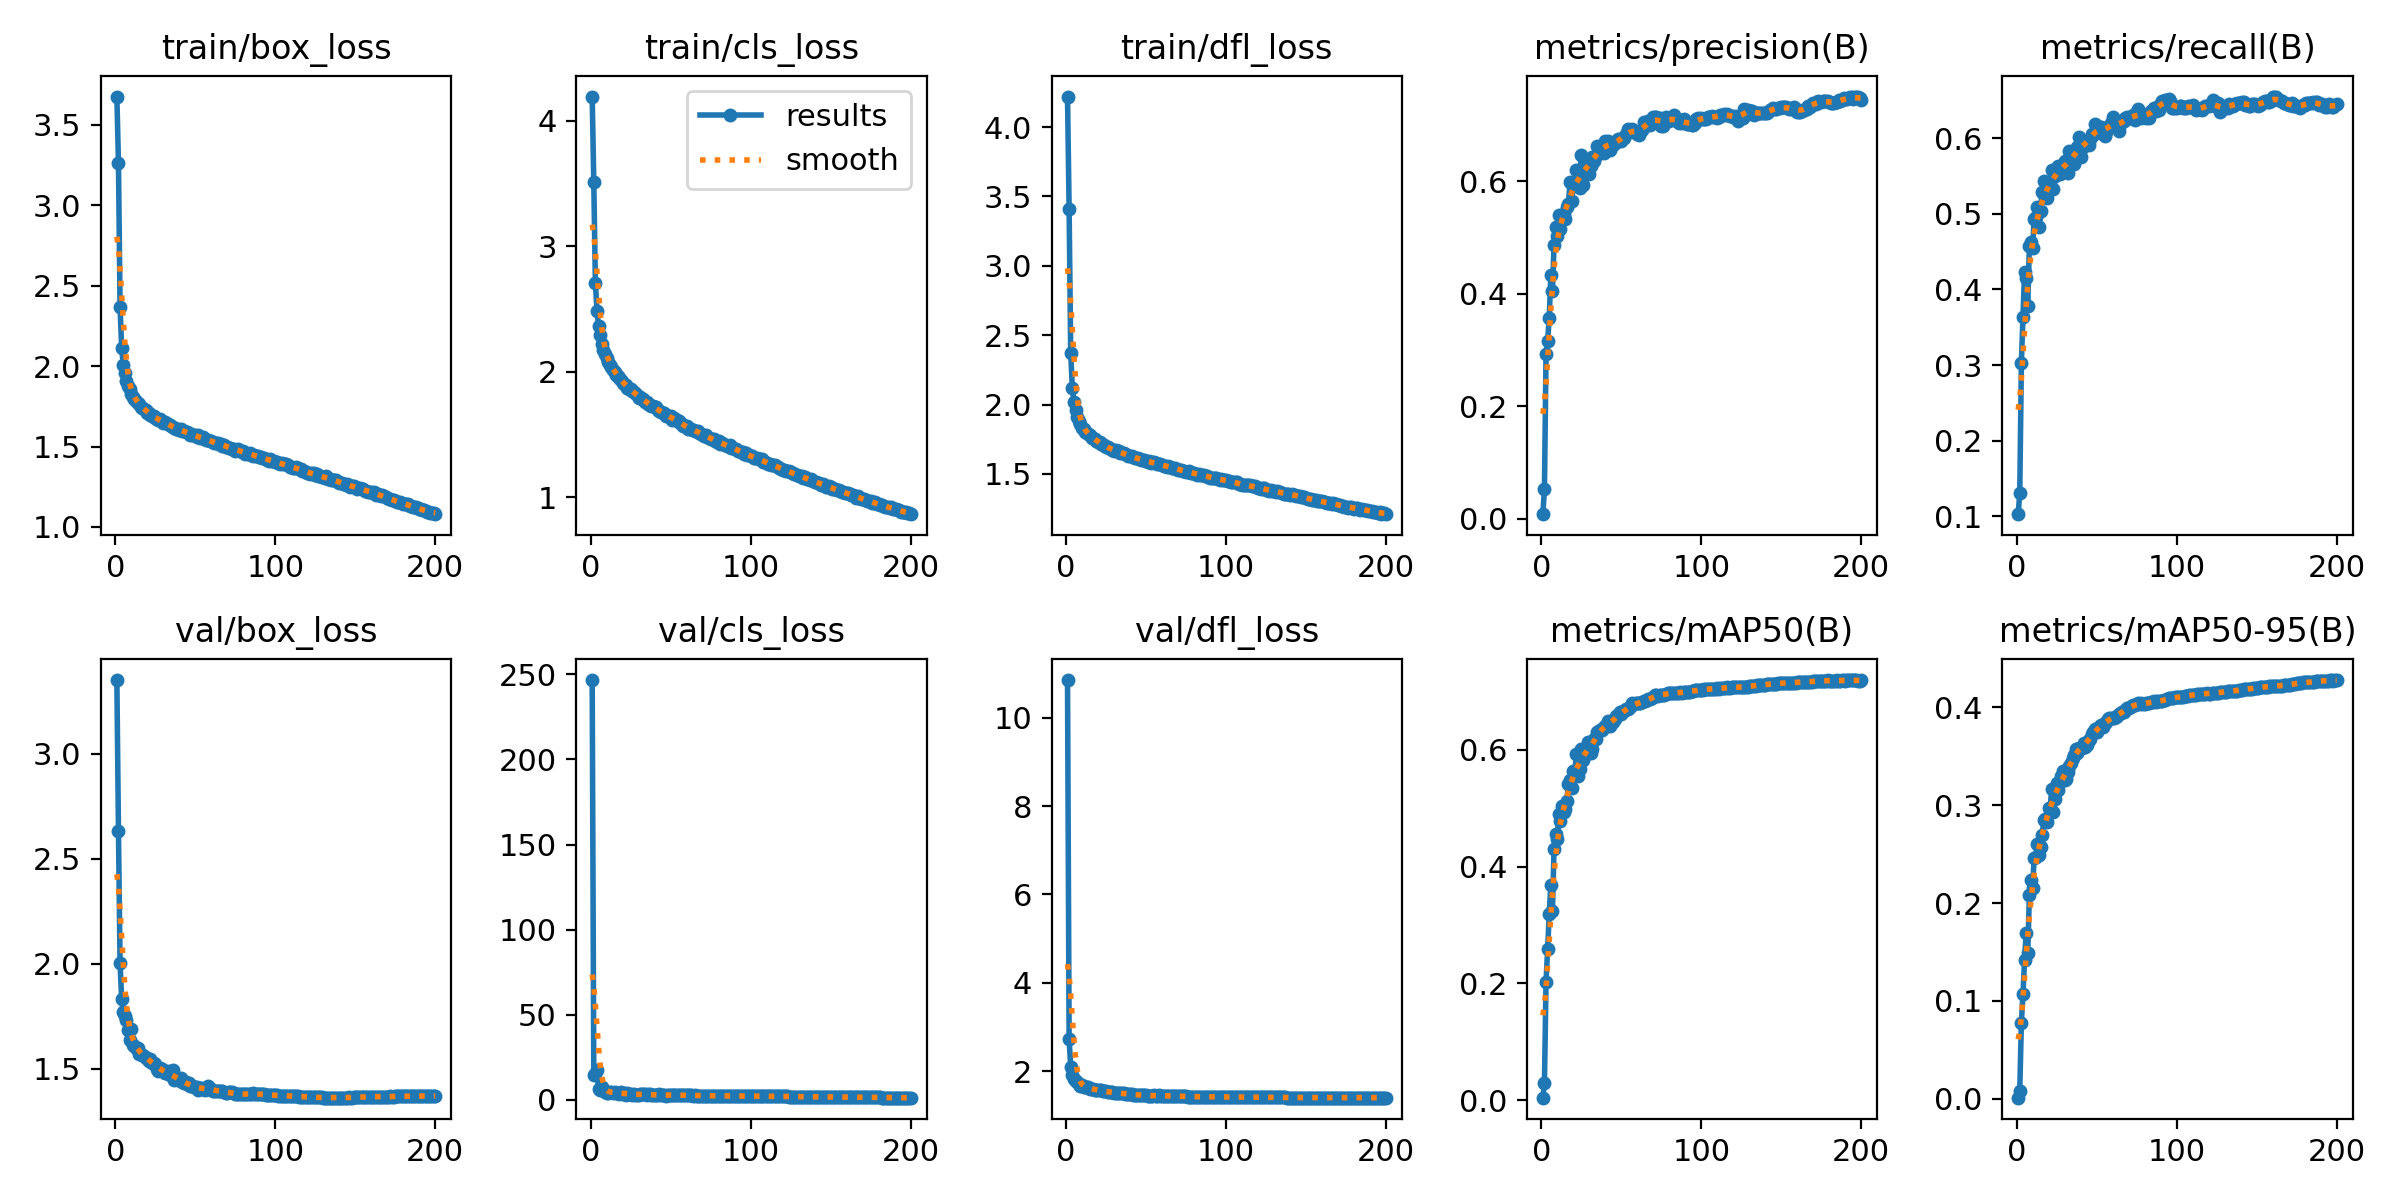
\includegraphics[width=\linewidth,height=.57\textheight,keepaspectratio]{images/reproduction/training_curves.png}
\end{column}
\end{columns}
\vspace{.1cm}\scriptsize 从随机初始化训练 200 epochs，batch 40，best.pt 在完整 valid split 上评估；本次验证由本地 RTX 4060、batch 4 完成，不能与论文 174 FPS 直接比较。
\paperref{Ultralytics results.csv 与完整 valid split 评估；输入 640 × 640}
\end{frame}

\begin{frame}{验证集诊断：PR 曲线与类别混淆}
\begin{columns}[T,onlytextwidth]
\begin{column}{.57\textwidth}
\centering
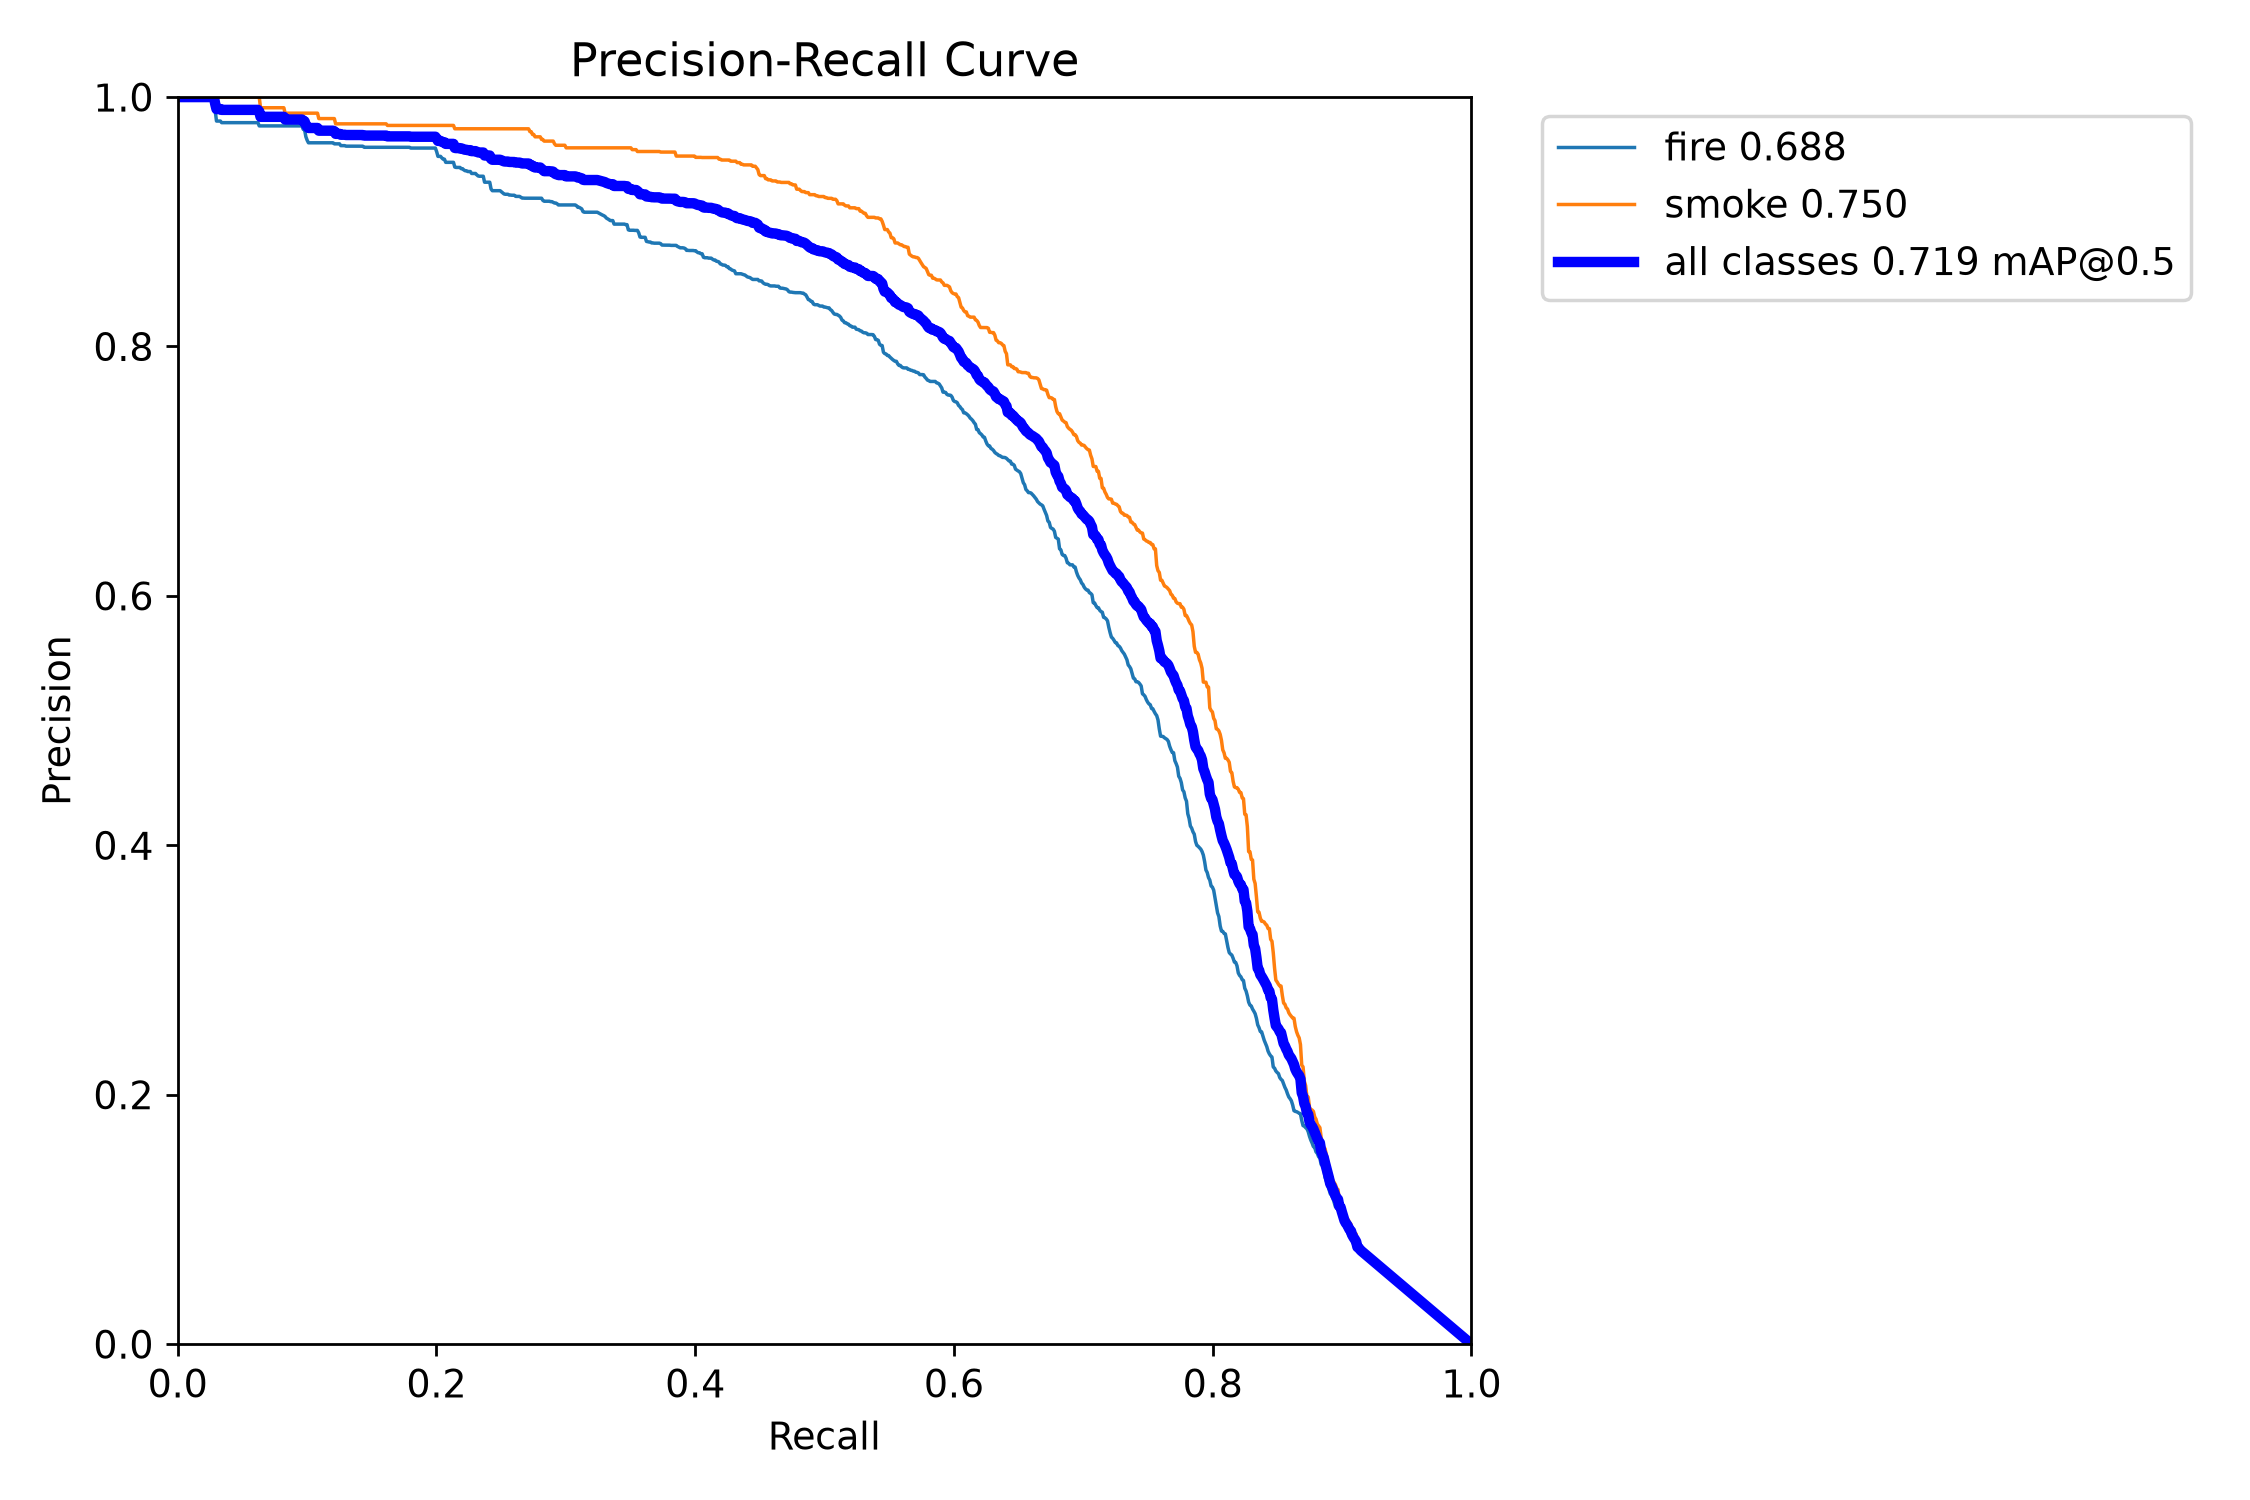
\includegraphics[width=\linewidth,height=.65\textheight,keepaspectratio]{images/reproduction/PR_curve.png}
\par\scriptsize Fire AP@0.5 = 68.8\%；Smoke AP@0.5 = 75.0\%。
\end{column}
\begin{column}{.40\textwidth}
\centering
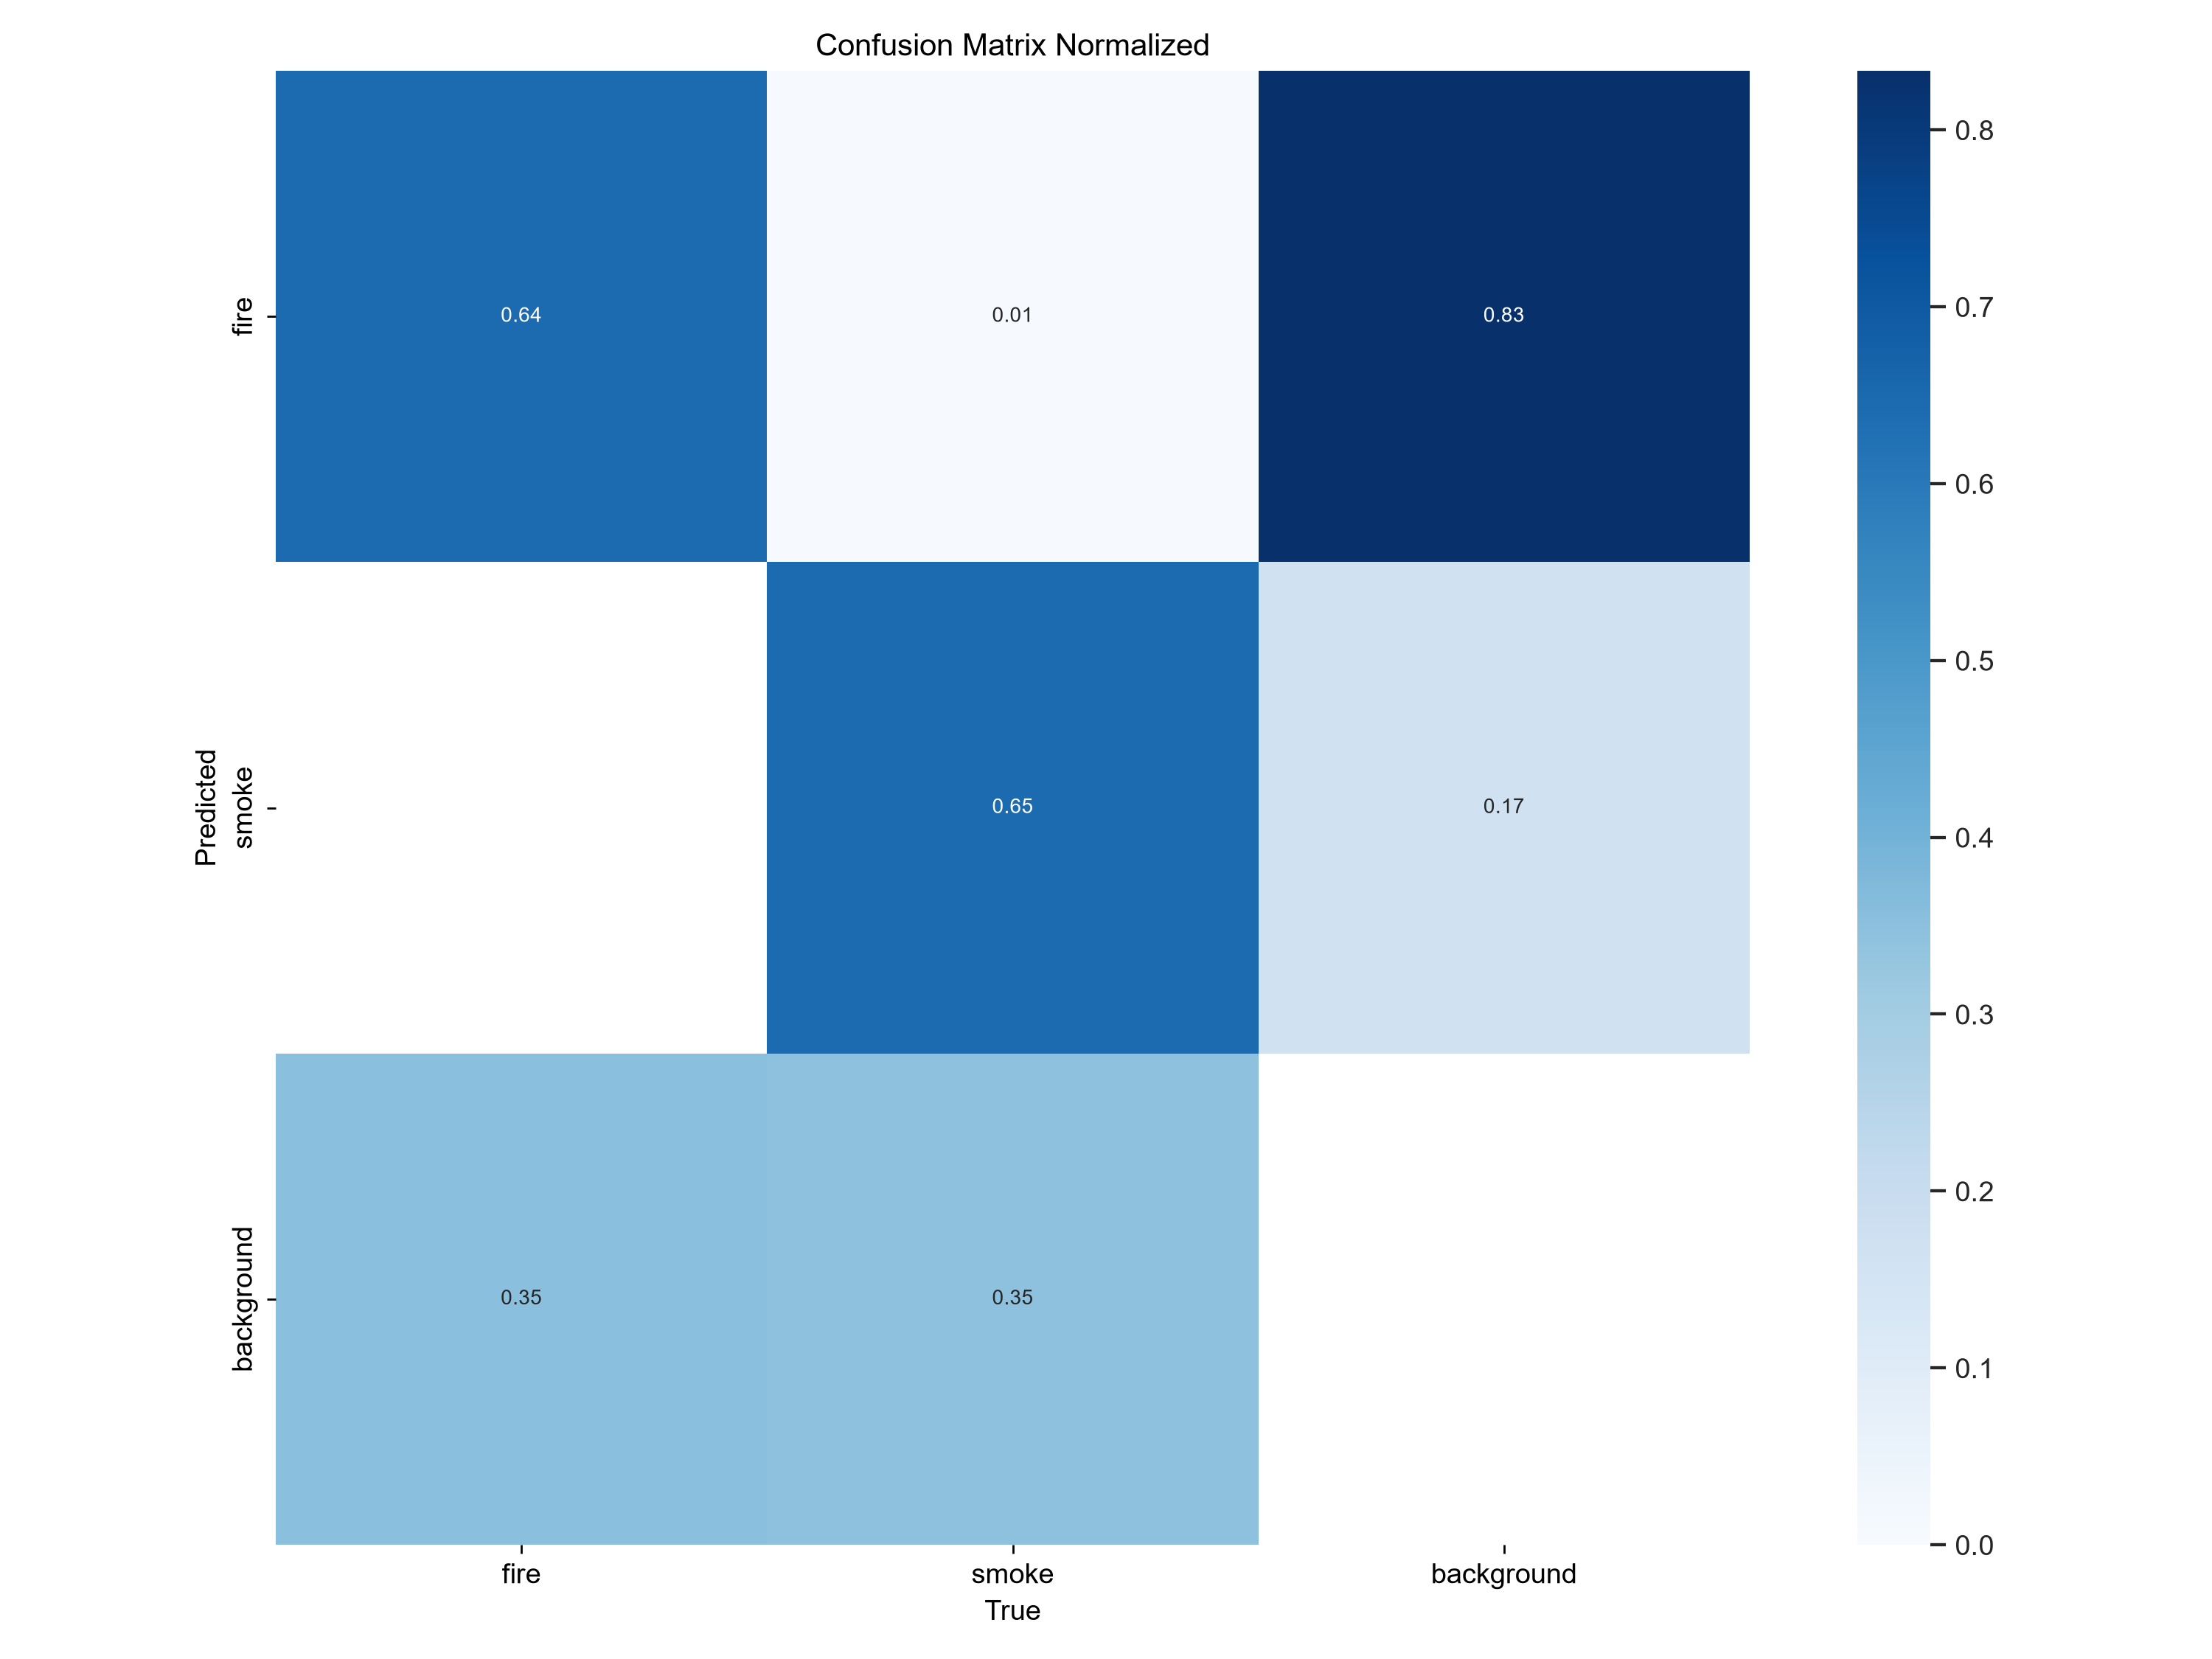
\includegraphics[width=\linewidth,height=.55\textheight,keepaspectratio]{images/reproduction/confusion_matrix_normalized.png}
\par\scriptsize 归一化混淆矩阵；背景行/列可见漏检与误报。
\end{column}
\end{columns}
\vfill\small Smoke 指标高于 Fire；后面的样例同时展示命中、漏检、类别混淆和背景误报。
\paperref{完整 valid split；best.pt；置信度阈值由验证流程选择}
\end{frame}

\begin{frame}{结论：论文同时改进模型结构和数据资源}
\begin{enumerate}
\item 火烟图像检测面临烟雾弱边缘、背景相似和远距离小目标等难点。
\item Finaldata 汇集 D-Fire 与网络图像；本地核查了 16,885 张图像的划分、类别与标签。
\item APConv 提取方向和尺度特征；C2f-AFF / ECN 融合特征；LSADetect 在多尺度上预测。
\item 论文报告准确率提升与 174 FPS；本次从头训练验证集 mAP@0.5 为 71.9\%，训练初始化不同，速度口径也不同。
\end{enumerate}
\vspace{.25cm}\textbf{汇报重点：}数据来源、样本与标签是否可信，和模型结构改动同样值得关注。
\end{frame}

\begin{frame}{可借鉴什么？后续还可以怎么改？}
\begin{columns}[T,onlytextwidth]
\begin{column}{.48\textwidth}
\begin{block}{可借鉴的思路}
\begin{itemize}
\item 先明确难例，再让模块针对具体困难设计。
\item 形状与方向特征、跨层融合、多尺度预测可以组合起来处理不同大小的火烟。
\item 数据清理和来源覆盖也是方法的一部分，不能只比较网络结构。
\end{itemize}
\end{block}
\end{column}
\begin{column}{.48\textwidth}
\begin{block}{值得继续验证的方向}
\begin{itemize}
\item 按拍摄地点或视频来源划分训练与测试，检验跨场景泛化。
\item 增加云、雾、蒸汽、扬尘、逆光等困难负样本，并单独报告误报。
\item 分别报告小烟、远距离目标和各场景指标，检查总体 mAP 是否掩盖弱项。
\item 若用于实际监控，再评估视频连续性、端侧延迟和功耗。
\end{itemize}
\end{block}
\end{column}
\end{columns}
\vspace{.2cm}\small 左侧是从论文方法抽象出的可迁移思路；右侧是后续研究建议，不是论文已经完成的实验。
\end{frame}

\begin{frame}{参考文献}
\small
\begin{thebibliography}{9}
\bibitem{dong2026} S. Dong, Y. Guo, Z. Wu, G. Xie, W. Xie, Y. Gu, and W. Xu.\newblock You only look once meets asymmetric pronged convolution: A unified framework for efficient fire and smoke detection.\newblock \emph{Engineering Applications of Artificial Intelligence}, 173:114484, 2026. doi:10.1016/j.engappai.2026.114484.
\bibitem{finaldata} 123dsb-ux.\newblock Finaldata: AEL-YOLO code and fire-smoke dataset.\newblock \url{https://github.com/123dsb-ux/Finaldata}.
\bibitem{dfire} P. V. A. B. de Ven\^ancio et al.\newblock An automatic fire detection system based on deep convolutional neural networks for low-power, resource-constrained devices.\newblock \emph{Neural Computing and Applications}, 2022.
\end{thebibliography}
\vfill\small 论文结构图与方法图来自原文；本次训练曲线、验证指标和对照样例来自本项目复现。
\end{frame}

\begin{frame}{谢谢，欢迎提问}
\centering
\vspace{1cm}
{\Large 火烟检测效果取决于模型，也取决于训练数据和评估方式。}
\vspace{.7cm}

\large Questions
\end{frame}

\appendix
\section{备份页}
\begin{frame}{备份：从 YAML 一行读懂网络结构}
\begin{itemize}
\item YAML 的一行形式：`[from, repeats, module, args]`。
\item `[-1, 1, Conv, [128, 3, 2]]`：接上一层，执行一次 128 通道、3×3、步长 2 卷积。
\item `[-1, 3, C2f\_iAFF, [256, True]]`：接上一层，重复三次 C2f\_iAFF。
\item `[[15,18,21], 1, Detect\_SA, [nc]]`：把三个尺度送入检测头。
\item 结构 YAML 负责搭网络；`best.pt` 才保存训练得到的模型参数。
\end{itemize}
\end{frame}

\begin{frame}{备份：论文模块名与仓库类名对照}
\centering
\vspace{3pt}
\renewcommand{\arraystretch}{1.25}
\begin{tabularx}{.93\textwidth}{l l X}
\toprule
论文表述 & 作者代码 / YAML & 作用\\ \midrule
APConv & `iAFF6.py`、`SAhead6.py` & 分解卷积核，组合方向与尺度特征\\
C2f-AFF & `C2f\_iAFF` & 将 APConv 接入 C2f，并加入注意力融合\\
ECN & `GSConv`、`VoVGSCSP`（`ECN.py`） & 轻量卷积和跨阶段融合\\
LSADetect & `Detect\_SA` & 多尺度预测分支加入 APConv 与 Self-Attention\\
\bottomrule
\end{tabularx}
\vspace{.25cm}\small 阅读复现代码时优先对照 YAML 中实际类名与模块定义，不只看配置文件名。
\end{frame}

\begin{frame}{备份：复现设置与论文结果的比较边界}
\begin{itemize}
\item 论文作者训练脚本：batch 16、pretrained=True、最多 200 epochs。
\item 本次服务器训练：batch 40、pretrained=False、200 epochs、seed 0。
\item 从头训练更符合当前用户的实验要求，但初始化不同会影响最终指标和收敛速度。
\item 报告时同时保留训练配置、软件版本、GPU、随机种子与完整验证指标。
\item 论文 174 FPS 是作者测速结果；不能直接当作本服务器的同口径速度。
\end{itemize}
\end{frame}

\begin{frame}{备份：常用评估指标怎么读}
\begin{itemize}
\item Precision：模型报出的目标里，有多少确实是目标。
\item Recall：图像里真实存在的目标，有多少被模型找到了。
\item AP@0.5：在 IoU=0.5 判定标准下，综合不同置信度阈值得到的类别检测表现。
\item mAP@0.5:0.95：综合更严格的多个 IoU 阈值，反映定位精度与分类效果。
\item FPS：特定设备与测速设置下每秒处理图像数；不等于端到端告警延迟。
\end{itemize}
\end{frame}

\section{本次验证集图像对照}
\begin{frame}{验证样例 1/8：多个火焰目标均被定位}
\centering
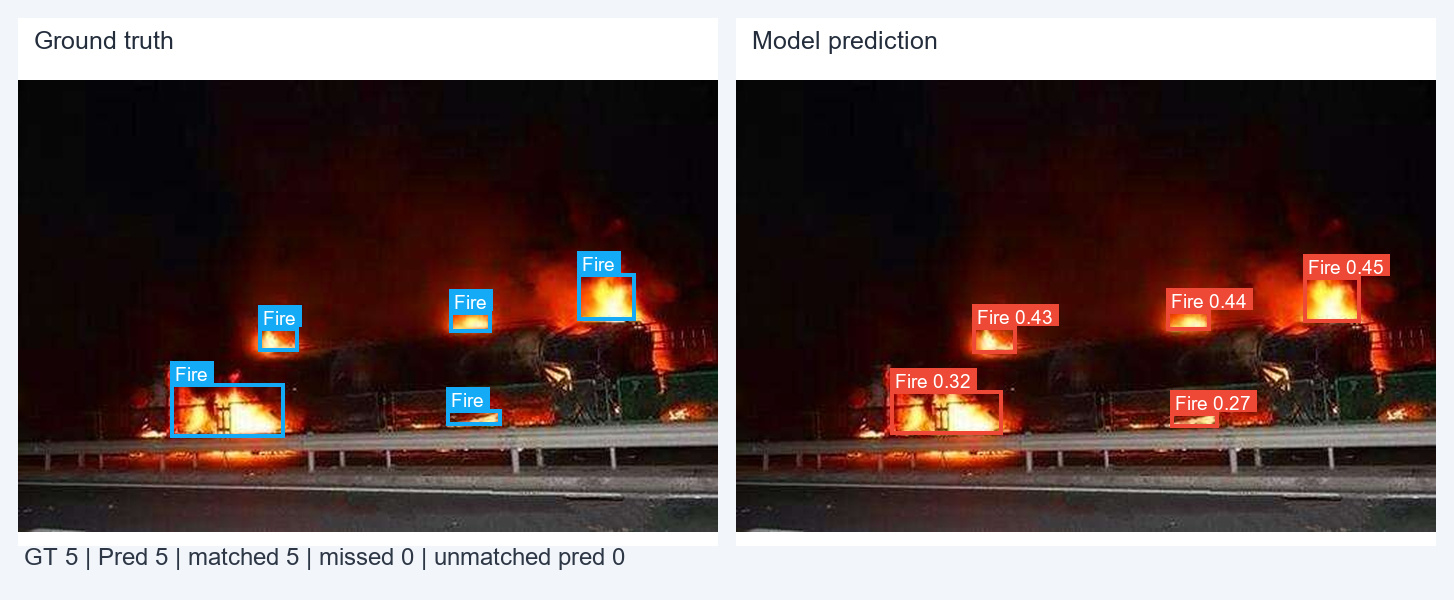
\includegraphics[width=.98\linewidth,height=.63\textheight,keepaspectratio]{images/reproduction/case_01_fire.jpg}
\par\vspace{.12cm}\small 5 个火焰标注框均有同类别预测框匹配，置信度为 0.27--0.45。
\paperref{Finaldata valid；best.pt；匹配条件：同类别且 IoU $\geq 0.5$}
\end{frame}

\begin{frame}{验证样例 2/8：火焰类别与位置都可能出错}
\centering
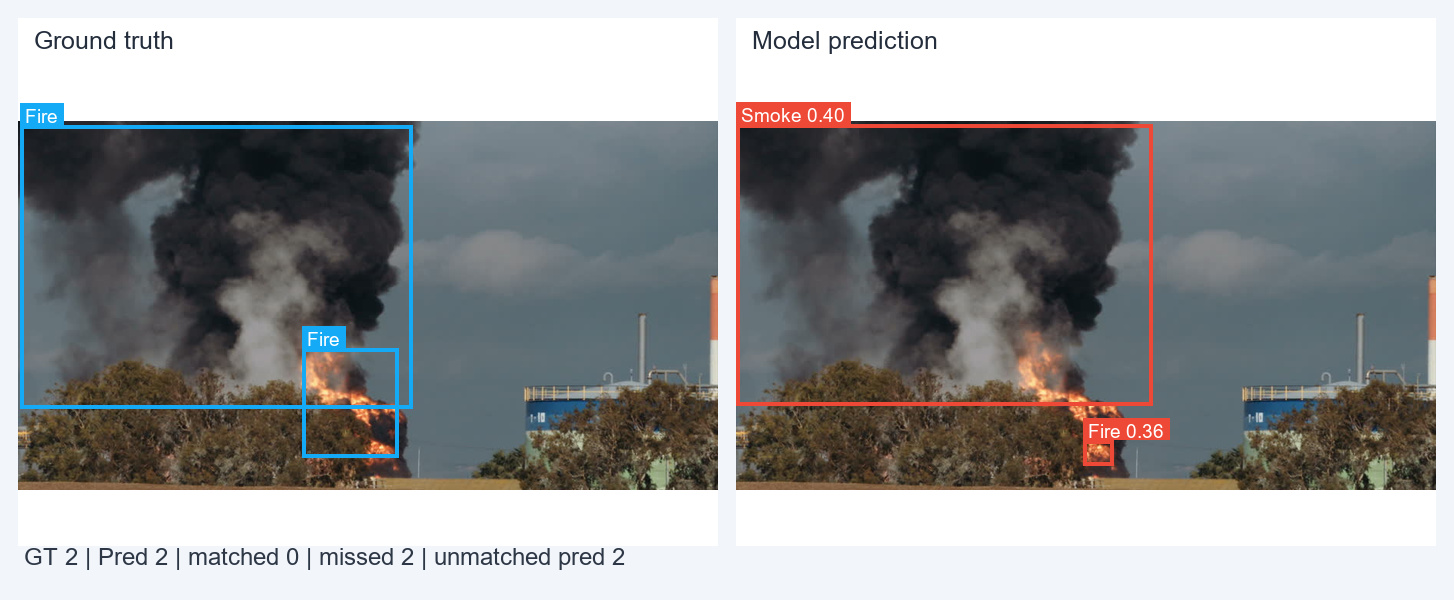
\includegraphics[width=.98\linewidth,height=.63\textheight,keepaspectratio]{images/reproduction/case_02_fire.jpg}
\par\vspace{.12cm}\small 标注为 2 个火焰框；模型给出 2 个预测，但类别或框位置未达到匹配标准。
\paperref{Finaldata valid；best.pt；红框为预测，蓝框为人工标注}
\end{frame}

\begin{frame}{验证样例 3/8：单个烟雾框被检出}
\centering
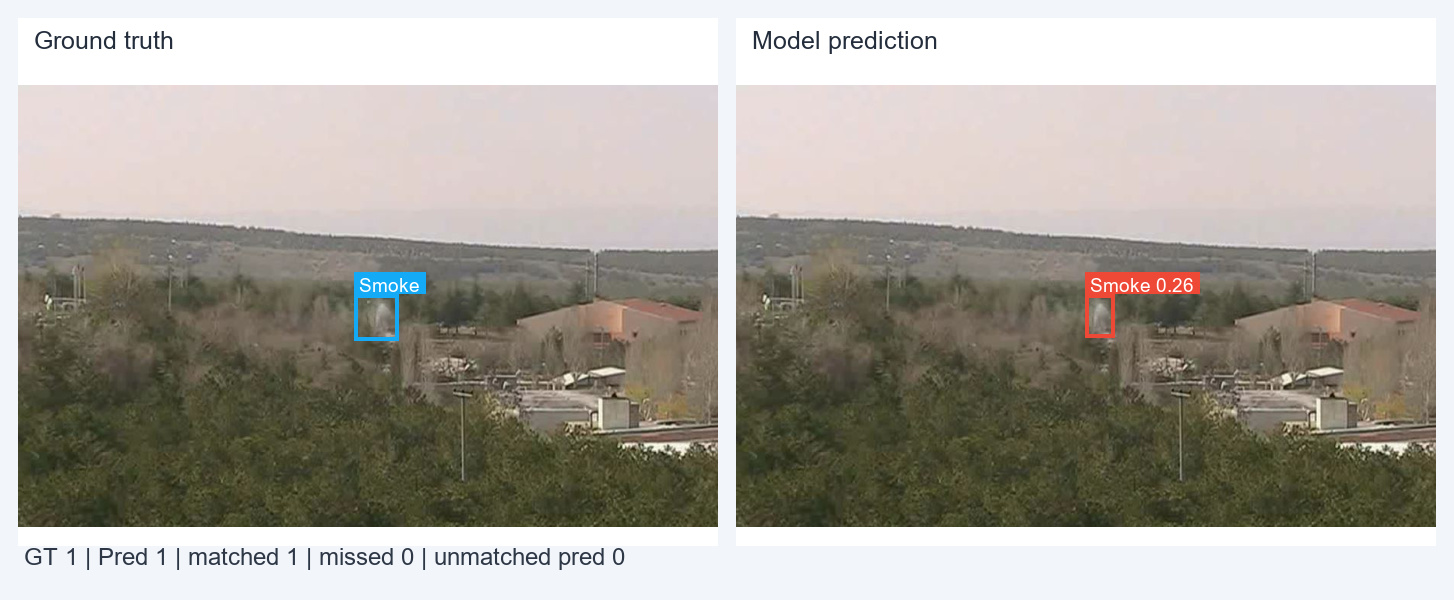
\includegraphics[width=.98\linewidth,height=.63\textheight,keepaspectratio]{images/reproduction/case_03_smoke.jpg}
\par\vspace{.12cm}\small 烟雾框匹配 IoU 为 0.61；置信度 0.26，接近本次展示阈值 0.25。
\paperref{Finaldata valid；best.pt；展示阈值 conf=0.25}
\end{frame}

\begin{frame}{验证样例 4/8：烟雾边界模糊时框偏差变大}
\centering
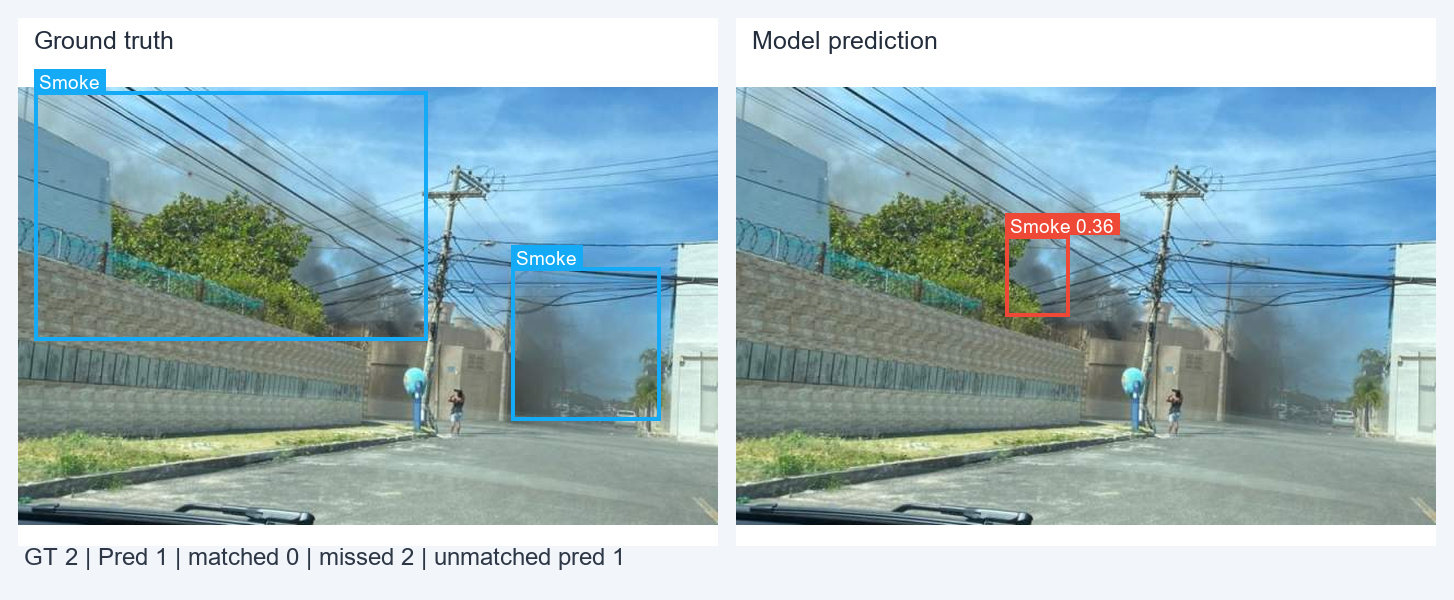
\includegraphics[width=.98\linewidth,height=.63\textheight,keepaspectratio]{images/reproduction/case_04_smoke.jpg}
\par\vspace{.12cm}\small 标注包含 2 个烟雾框；模型预测 1 框，但没有达到 IoU 0.5 的匹配条件。
\paperref{Finaldata valid；best.pt；未匹配不等同于人工标注一定正确}
\end{frame}

\begin{frame}{验证样例 5/8：火焰与烟雾同框}
\centering
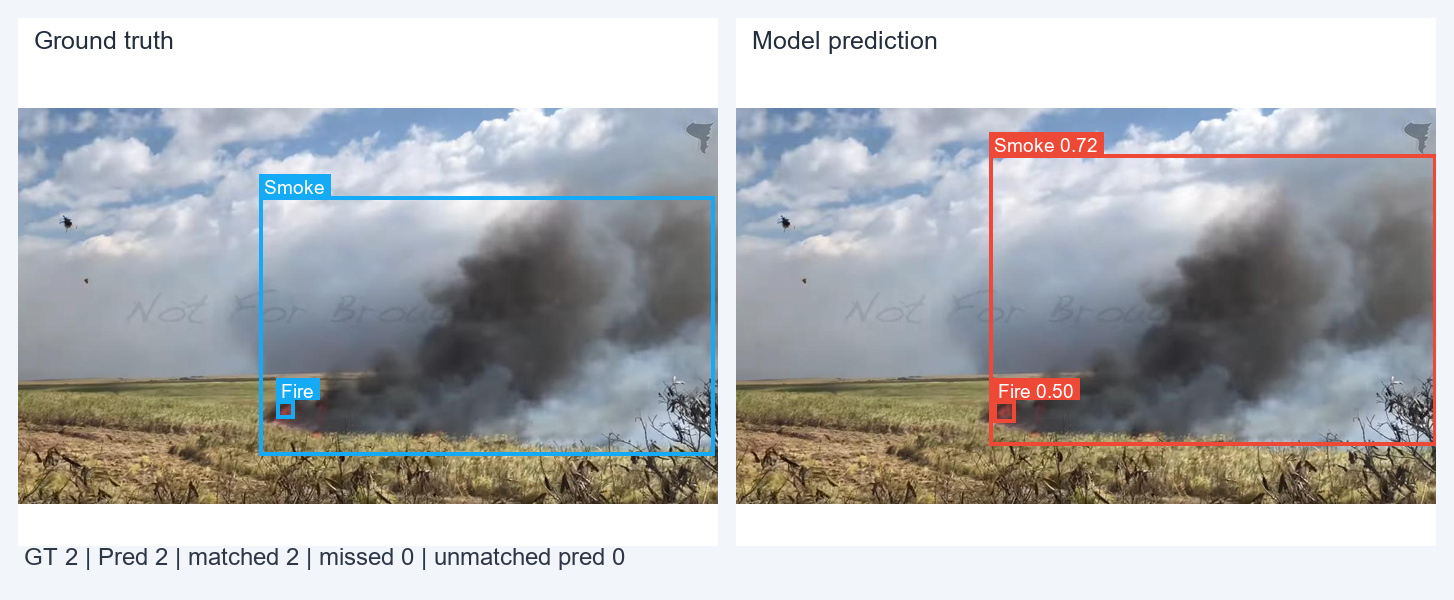
\includegraphics[width=.98\linewidth,height=.63\textheight,keepaspectratio]{images/reproduction/case_05_mixed.jpg}
\par\vspace{.12cm}\small 两个类别各有标注框，模型均检出；火焰框 IoU 0.62，烟雾框 IoU 0.80。
\paperref{Finaldata valid；best.pt；同类别且 IoU $\geq 0.5$ 计为匹配}
\end{frame}

\begin{frame}{验证样例 6/8：浓烟可能被分成错误类别}
\centering
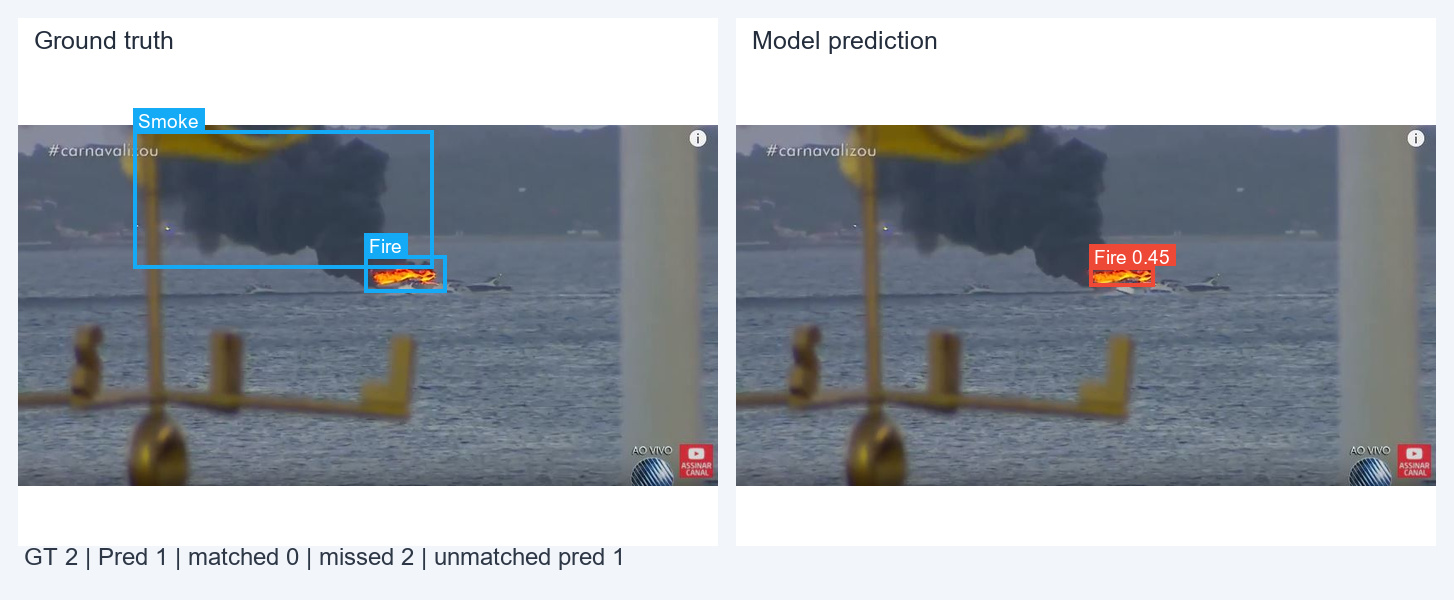
\includegraphics[width=.98\linewidth,height=.63\textheight,keepaspectratio]{images/reproduction/case_06_mixed.jpg}
\par\vspace{.12cm}\small 真实标注为火焰与烟雾；模型只预测 1 个 Fire 框，两个标注均未匹配。
\paperref{Finaldata valid；best.pt；展示阈值 conf=0.25}
\end{frame}

\begin{frame}{验证样例 7/8：负样本没有触发检测}
\centering
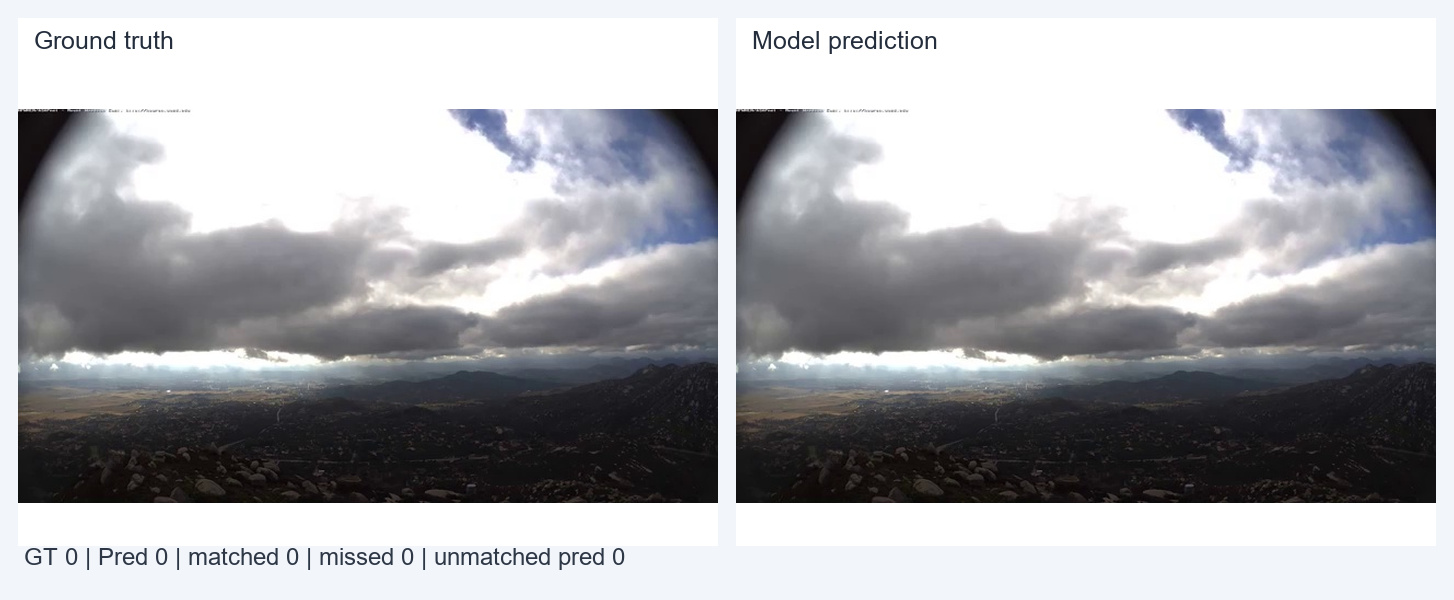
\includegraphics[width=.98\linewidth,height=.63\textheight,keepaspectratio]{images/reproduction/case_07_background.jpg}
\par\vspace{.12cm}\small 该验证图片没有火烟标注，模型也未输出检测框。
\paperref{Finaldata valid 的无目标背景图；best.pt}
\end{frame}

\begin{frame}{验证样例 8/8：负样本误报火焰}
\centering
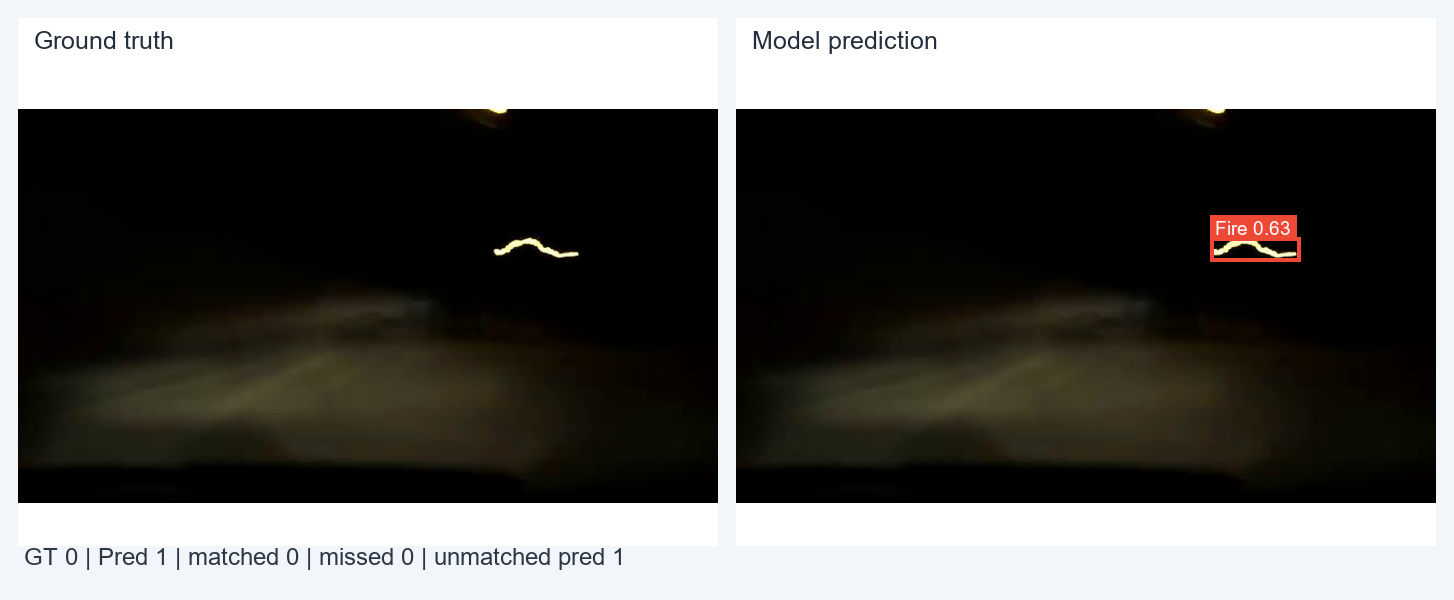
\includegraphics[width=.98\linewidth,height=.63\textheight,keepaspectratio]{images/reproduction/case_08_background.jpg}
\par\vspace{.12cm}\small 该图片没有火烟标注，模型却输出一个 Fire 框；背景负样本仍需要扩充和专项评估。
\paperref{Finaldata valid 的无目标背景图；best.pt；展示阈值 conf=0.25}
\end{frame}
\end{document}






